\documentclass[
	% -- opções da classe memoir --
	article,			% indica que é um artigo acadêmico
	11pt,				% tamanho da fonte
	oneside,			% para impressão apenas no recto. Oposto a twoside
	a4paper,			% tamanho do papel.
	% -- opções da classe abntex2 --
	%chapter=TITLE,		% títulos de capítulos convertidos em letras maiúsculas
	%section=TITLE,		% títulos de seções convertidos em letras maiúsculas
	%subsection=TITLE,	% títulos de subseções convertidos em letras maiúsculas
	%subsubsection=TITLE % títulos de subsubseções convertidos em letras maiúsculas
	% -- opções do pacote babel --
	english,			% idioma adicional para hifenização
	brazil,				% o último idioma é o principal do documento
	sumario=tradicional
	]{abntex2}


% ---
% PACOTES
% ---

% ---
% Pacotes fundamentais
% ---
\usepackage{lmodern}			% Usa a fonte Latin Modern
\usepackage[T1]{fontenc}		% Selecao de codigos de fonte.
\usepackage[utf8]{inputenc}		% Codificacao do documento (conversão automática dos acentos)
\usepackage{indentfirst}		% Indenta o primeiro parágrafo de cada seção.
\usepackage{nomencl} 			% Lista de simbolos
\usepackage{color}				% Controle das cores
\usepackage{graphicx}			% Inclusão de gráficos
\usepackage{microtype} 			% para melhorias de justificação
% ---
\usepackage{hyperref}
\usepackage{listings}
\usepackage{xcolor}
\usepackage{tcolorbox}
\usepackage{siunitx}
\usepackage{pdfpages}
% ---
% Pacotes adicionais, usados apenas no âmbito do Modelo Canônico do abnteX2
% ---
\usepackage{lipsum}				% para geração de dummy text
% ---

% ---
% Pacotes de citações
% ---
\usepackage[brazilian,hyperpageref]{backref}	 % Paginas com as citações na bibl
\usepackage[alf, abnt-emphasize=bf]{abntex2cite} % Estilo ABNT alfabético% ---

% ---
% Configurações do pacote backref
% Usado sem a opção hyperpageref de backref
\renewcommand{\backrefpagesname}{Citado na(s) página(s):~}
% Texto padrão antes do número das páginas
\renewcommand{\backref}{}
% Define os textos da citação
\renewcommand*{\backrefalt}[4]{
	\ifcase #1 %
		Nenhuma citação no texto.%
	\or
		Citado na página #2.%
	\else
		Citado #1 vezes nas páginas #2.%
	\fi}%
% ---

% --- Informações de dados para CAPA e FOLHA DE ROSTO ---
\titulo{ESTUDO E RESOLUÇÃO DO CICLO DE RANKINE COM MODIFICAÇÕES}
\tituloestrangeiro{}

\autor{
João Alex Arruda da Silva
\\[0.5cm]
Hanna Rodrigues Ferreira}

\local{Brasil}
\data{Fevereiro, 2025}
% ---

% ---
% Configurações de aparência do PDF final

% alterando o aspecto da cor azul
\definecolor{blue}{RGB}{41,5,195}

% informações do PDF
\makeatletter
\hypersetup{
     	%pagebackref=true,
		pdftitle={\@title},
		pdfauthor={\@author},
    	pdfsubject={Modelo de artigo científico com abnTeX2},
	    pdfcreator={LaTeX with abnTeX2},
		pdfkeywords={abnt}{latex}{abntex}{abntex2}{atigo científico},
		colorlinks=true,       		% false: boxed links; true: colored links
    	linkcolor=blue,          	% color of internal links
    	citecolor=blue,        		% color of links to bibliography
    	filecolor=magenta,      		% color of file links
		urlcolor=blue,
		bookmarksdepth=4
}
\makeatother
% ---

% ---
% compila o indice
% ---
\makeindex
% ---

% ---
% Altera as margens padrões
% ---
\setlrmarginsandblock{3cm}{3cm}{*}
\setulmarginsandblock{3cm}{3cm}{*}
\checkandfixthelayout
% ---

% ---
% Espaçamentos entre linhas e parágrafos
% ---

% O tamanho do parágrafo é dado por:
\setlength{\parindent}{1.3cm}

% Controle do espaçamento entre um parágrafo e outro:
\setlength{\parskip}{0.2cm}  % tente também \onelineskip

% Espaçamento simples
\SingleSpacing


% ----
% Início do documento
% ----
\begin{document}

% Seleciona o idioma do documento (conforme pacotes do babel)
%\selectlanguage{english}
\selectlanguage{brazil}

% Retira espaço extra obsoleto entre as frases.
\frenchspacing

% ----------------------------------------------------------
% ELEMENTOS PRÉ-TEXTUAIS
% ----------------------------------------------------------

%---
%
% Se desejar escrever o artigo em duas colunas, descomente a linha abaixo
% e a linha com o texto ``FIM DE ARTIGO EM DUAS COLUNAS''.
% \twocolumn[    		% INICIO DE ARTIGO EM DUAS COLUNAS
%
%---

% página de titulo principal (obrigatório)
\maketitle


% titulo em outro idioma (opcional)



% resumo em português
\begin{resumoumacoluna}
	Este trabalho analisa o ciclo de Rankine, muito utilizado na geração de energia
	nas usinas termelétricas que operam com vapor. São abordados seus processos
	básicos e modificações que aumentam a eficiência térmica, como superaquecimento,
	reaquecimento, regeneração e entre outras. A metodologia inclui uma revisão teórica
	e um estudo de caso em que realizamos cálculos de eficiência térmica, trabalho das
	turbinas e bombas, vazão mássica e construção dos diagramas T-s. Além disso, é
	realizado uma análise paramétrica do desempenho do ciclo. Os resultados nos
	mostram que tais modificações melhoram a eficiência, mas que é necessário um estudo aprofundado.

 \vspace{\onelineskip}

 \noindent
 \textbf{Palavras-chave}: Ciclo de Rankine. Eficiência térmica. Superaquecimento. Diagrama T-s.
\end{resumoumacoluna}

% ----------------------------------------------------------
% ELEMENTOS TEXTUAIS
% ----------------------------------------------------------
\textual

% ----------------------------------------------------------
% Introdução
% ----------------------------------------------------------
\section{Introdução}

Segundo \cite{moran-2018}, o ciclo de Rankine é a estrutura fundamental das usinas termelétricas que operam com vapor. Este é um dos principais ciclos termodinâmicos utilizados na engenharia mecânica para conversão de calor em trabalho, sendo a base para o funcionamento de usinas termoelétricas e outras instalações de geração de energia. Esse ciclo opera com um fluido de trabalho, geralmente água, que passa por processos de aquecimento, expansão, resfriamento e compressão.

Para melhorar a eficiência do Ciclo de Rankine, diversas modificações são adotadas, como o superaquecimento, o reaquecimento e o uso de ciclos supercríticos. Essas modificações têm o objetivo de aumentar a eficiência térmica e reduzir perdas energéticas, tornando as plantas de geração mais sustentáveis e econômicas.

Este trabalho pretende analisar detalhadamente o ciclo de Rankine e suas variações, visando aprofundar o conhecimento sobre sistemas térmicos voltados à produção de energia. Para isso, será realizada uma revisão teórica robusta dos princípios termodinâmicos envolvidos, seguida da aplicação desses conceitos em um estudo de caso prático, que abordará técnicas como reaquecimento, expansão em dois estágios e regeneração térmica.

\section{Revisão bibliográfica}

\subsection{Definição do ciclo de Rankine}

O Ciclo de Rankine é um ciclo termodinâmico idealizado que descreve o funcionamento de uma usina termelétrica convencional. Esse ciclo é composto por quatro processos termodinâmicos: compressão, aquecimento, expansão e resfriamento. A Figura \ref{fig:esquema-simplificado-ciclo-rankine} ilustra o diagrama de um ciclo de Rankine básico.

\begin{figure}[h]
	\centering
	\caption{Esquema simplificado e o diagrama T-S do ciclo Rankine}
	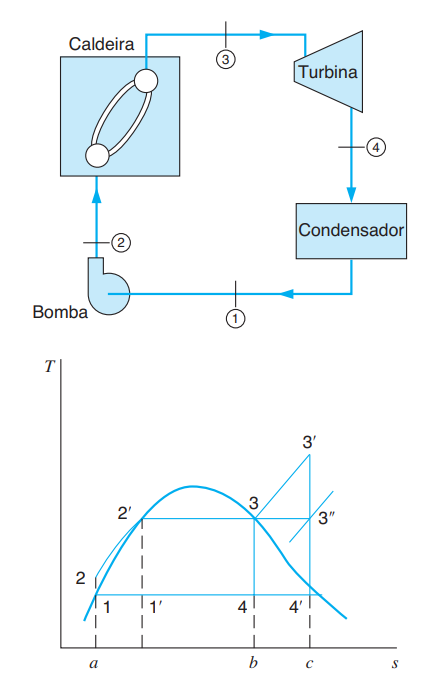
\includegraphics[width=0.7\textwidth]{./images/Esquema simplificado e o diagrama T-S do ciclo Rankine.png}
	\label{fig:esquema-simplificado-ciclo-rankine}
	\fonte{Adaptado de \cite{borgnakke-2020}}
\end{figure}

O fluido de trabalho fica sujeito à seguinte sequência de processos reversíveis internamente: \cite{borgnakke-2020}

\begin{itemize}
	\item \textbf{Processo 1-2}: Processo de bombeamento adiabático reversível na bomba.
	\item \textbf{Processo 2-3}: Transferência de calor a pressão constante na caldeira.
	\item \textbf{Processo 3-4}: Expansão adiabática reversível na turbina (ou em outra máquina motora, tal como a máquina a vapor).
	\item \textbf{Processo 4-1}: Transferência de calor a pressão constante no condensador.
\end{itemize}

Ao desconsiderar as variações de energia cinética e potencial, as trocas de calor e o trabalho líquido do sistema podem ser visualizados como áreas específicas no diagrama temperatura-entropia (T-s). O calor absorvido pelo fluido de trabalho corresponde à área delimitada pelos pontos a-2-2'-3-b-a, enquanto o calor rejeitado pelo fluido é representado pela área a-1-4-b-a. Aplicando a primeira lei da termodinâmica, conclui-se que o trabalho líquido é equivalente à diferença entre essas duas áreas, ou seja, corresponde à região 1-2-2'-3-4-1 no diagrama \cite{borgnakke-2020}.

Na análise do ciclo Rankine, é útil considerar que o rendimento depende da temperatura média na qual o calor é fornecido e da temperatura média na qual o calor é rejeitado. Qualquer variação que aumente a temperatura média na qual o calor é fornecido, ou que diminua a temperatura média na qual o calor é rejeitado, aumentará o rendimento do ciclo Rankine.

\subsection{Componentes Básicos}

Independentemente de um modelo detalhado ou simplificado de usina a vapor baseada no ciclo Rankine, os fundamentos termodinâmicos (conservação de massa/energia, segunda lei e dados termodinâmicos) aplicam-se tanto aos componentes individuais (turbinas, bombas, trocadores de calor) quanto ao ciclo global.

Focando no subsistema mostrado na Figura \ref{fig:planta-exemplo}, modelam-se os quatro componentes principais: turbina, condensador, bomba e caldeira, com água como fluido de trabalho. Usinas a combustíveis fósseis são analisadas como referência, mas os princípios valem para outros tipos.

\begin{figure}[h]
	\centering
	\caption{Planta de potência a vapor acionada por combustível fóssil}
	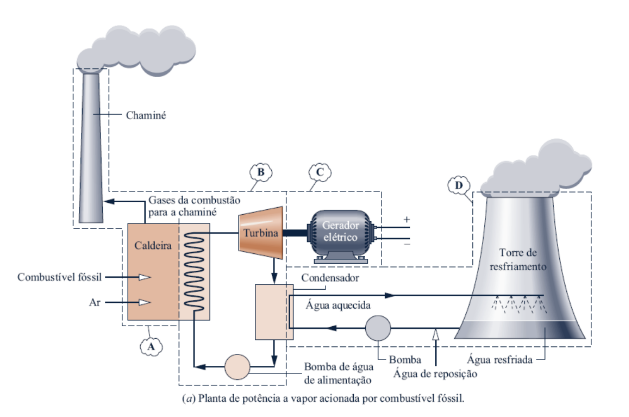
\includegraphics[width=1.0\textwidth]{./images/planta-exemplo.png}
	\label{fig:planta-exemplo}
	\fonte{\
	cite{moran-2018}}
\end{figure}

No diagrama da Fig. 2, trabalho e calor são positivos conforme as setas, para simplificar a análise usamos algumas hipóteses frequentes, conforme descrito abaixo:
\begin{itemize}
	\item R. P. em todos os componentes.
	\item Energia potencial e cinética desprezível.
    \item Perdas de pressão na caldeira e no condensador desprezíveis.
    \item Bombas e turbinas são consideradas isentrópicas.
\end{itemize}

Será mostrado a seguir a modelagem do ciclo para cada componente do ciclo Rankine, conforme é exibido por \citeonline{moran-2018}

\subsubsection{Turbina}

A turbina é o componente que converte a energia térmica do vapor em trabalho mecânico. O vapor entra na turbina com uma pressão e temperatura elevadas e sai com pressão e temperatura menores. O trabalho líquido da turbina é a diferença entre o trabalho de entrada e saída, conforme a equação \ref{eq:trabalho-turbina}.

\begin{equation}
	\dot{W}_{\text{turbina}} = \dot{m}(h_1 - h_2)
	\label{eq:trabalho-turbina}
\end{equation}

\subsubsection{Condensador}

O condensador é o componente que converte o vapor em água líquida, rejeitando calor para o ambiente. O calor rejeitado pelo condensador é a diferença entre o calor de entrada e saída, conforme a equação \ref{eq:calor-condensador}.

\begin{equation}
	\dot{Q}_{\text{condensador}} = \dot{m}(h_2 - h_3)
	\label{eq:calor-condensador}
\end{equation}

\subsubsection{Bomba}

A bomba é o componente que comprime a água líquida, aumentando sua pressão. O trabalho líquido da bomba é a diferença entre o trabalho de entrada e saída, conforme a equação \ref{eq:trabalho-bomba}.

\begin{equation}
	\dot{W}_{\text{bomba}} = \dot{m}(h_4 - h_3)
	\label{eq:trabalho-bomba}
\end{equation}

\subsubsection{Caldeira}

A caldeira é o componente que converte a água líquida em vapor, absorvendo calor do ambiente. O calor absorvido pela caldeira é a diferença entre o calor de entrada e saída, conforme a equação \ref{eq:calor-caldeira}.

\begin{equation}
	\dot{Q}_{\text{caldeira}} = \dot{m}(h_1 - h_2)
	\label{eq:calor-caldeira}
\end{equation}

\subsection{Parâmetros de Desempenho}

\subsubsection{Eficiência Térmica}

A eficiência térmica do ciclo Rankine é dada pela razão entre o trabalho líquido produzido e o calor fornecido na caldeira, conforme a equação \ref{eq:eficiencia-termica}.

\begin{equation}
	\eta = \frac{\dot{W}_{\text{turbina}}}{\dot{Q}_{\text{caldeira}}}
	\label{eq:eficiencia-termica}
\end{equation}

\subsubsection{Taxa de Calor}

A taxa de calor representa a quantidade de energia térmica fornecida ao sistema (geralmente medida em Btu) necessária para gerar uma unidade de trabalho útil produzido pelo ciclo (normalmente expresso em kWh). Por isso, ela é definida como a razão entre a energia térmica consumida e o trabalho líquido gerado, com unidades de Btu/kWh. Essa taxa tem uma relação inversa com a eficiência termodinâmica do ciclo: quanto maior a eficiência, menor a quantidade de calor requerida para produzir a mesma quantidade de trabalho.

\subsubsection{Back work ratio}

\begin{figure}[h]
	\centering
	\caption{Planta de potência a vapor acionada por combustível fóssil}
	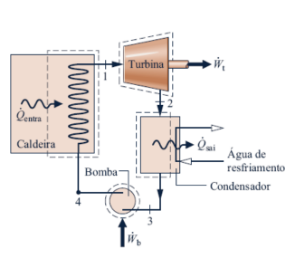
\includegraphics[width=0.5\textwidth]{./images/trabalho-realizado.png}
	\label{fig:trabalho-realizado}
	\fonte{\cite{moran-2018}}
\end{figure}

O back work ratio (bwr) é um parâmetro que quantifica a relação entre o trabalho consumido pela bomba e o trabalho gerado pela turbina no ciclo de potência. Para o sistema da Figura \ref{fig:trabalho-realizado}, usando as equações já definidas para o trabalho da bomba e da turbina, o bwr é calculado pela equação \ref{eq:bwr}.

\begin{equation}
	\text{bwr} = \frac{\dot{W}_{\text{bomba}}}{\dot{W}_{\text{turbina}}}
	\label{eq:bwr}
\end{equation}

\subsection{Aplicações do Ciclo de Rankine}

Dentre os sete tipos de usinas de energia que operam com base em ciclos termodinâmicos, seis estão diretamente vinculadas ao ciclo de Rankine. Esse ciclo é o elemento fundamental das usinas termelétricas a vapor, servindo como modelo central para conversão de calor em trabalho mecânico ou elétrico. Sua versatilidade permite aplicações em sistemas que vão desde usinas nucleares e movidas a combustíveis fósseis até fontes renováveis, como geotérmica e solar térmica, consolidando-o como pilar da geração de energia em larga escala.

A Figura \ref{fig:etn} mostra a turbina de Angra 2, uma usina nuclear que opera com base no ciclo de Rankine. A usina é composta por um reator nuclear, que gera calor, e uma turbina a vapor, que converte esse calor em energia elétrica. O ciclo de Rankine é responsável por transferir o calor do reator para a turbina, garantindo a eficiência do processo.

\begin{figure}[h]
	\centering
	\caption{Turbina de Angra 2}
	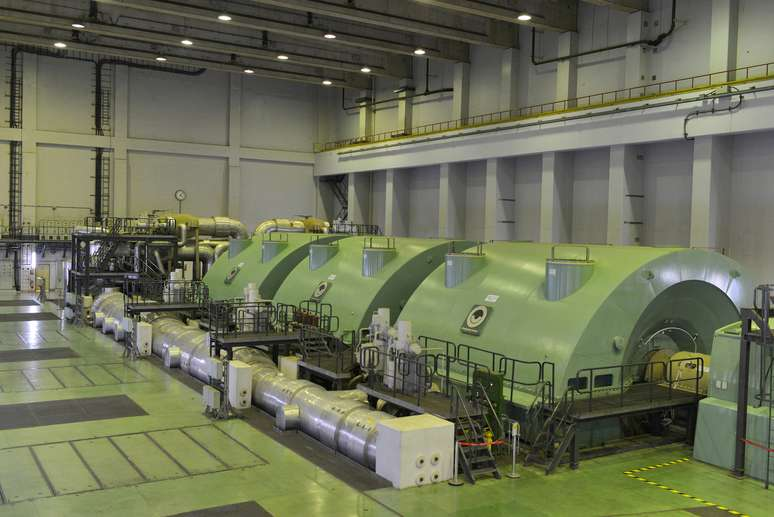
\includegraphics[width=0.7\textwidth]{./images/etn.jpg}
	\label{fig:etn}
	\fonte{\cite{Eletronuclear_Imagem_Angra}}
\end{figure}

\section{Parâmetros de influência na eficiência do ciclo de Rankine}

\subsection{Efeitos Da Pressão E Da Temperatura No Ciclo Rankine}

No ciclo Rankine, a pressão e a temperatura afetam diretamente o rendimento e o trabalho líquido realizado no ciclo. Em seguida, examinam-se os principais impactos dessas variáveis, juntamente com suas respectivas representações gráficas.

\subsection{Efeito da Pressão na Saída da Turbina}

No diagrama T-s da Figura \ref{fig:efeito-pressao}, observa-se o efeito da redução da pressão na saída da turbina, de P4 para P4'. Essa redução causa uma diminuição na temperatura na qual o calor é rejeitado. O aumento do trabalho líquido é representado pela área 1-4-4'-1'-2-2'-1, enquanto o aumento do calor transferido ao fluido corresponde à área a'-2'-2-a. Como essas duas áreas são aproximadamente iguais, o rendimento do ciclo aumenta, devido à redução da temperatura média de rejeição de calor. A redução da pressão também diminui o título do vapor na saída da turbina. Se a umidade ultrapassar 10\%, pode ocorrer erosão das palhetas e queda na eficiência \cite{borgnakke-2020}.

\begin{figure}[h]
	\centering
	\caption{Efeito da pressão de descarga da turbina sobre o rendimento do ciclo Rankine}
	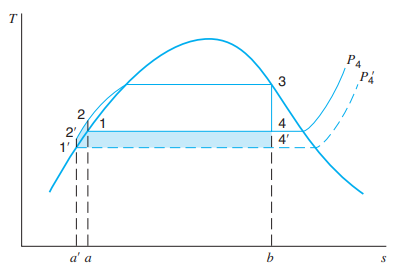
\includegraphics[width=0.4\textwidth]{./images/efeito-pressao.png}
	\label{fig:efeito-pressao}
	\fonte{\cite{borgnakke-2020}}
\end{figure}

\subsubsection{Efeito do Superaquecimento do Vapor}

Na Figura \ref{fig:efeito-vapor}, é mostrado o efeito do superaquecimento do vapor. O trabalho líquido aumenta correspondendo à área 3-3'-4'-4-3, e o calor transferido na caldeira aumenta com a área 3-3'-b'-b-3. Como a relação entre essas áreas é maior que a relação entre o trabalho líquido e o calor fornecido no restante do ciclo, o superaquecimento do vapor resulta em um aumento do rendimento do ciclo Rankine. O superaquecimento aumenta a temperatura média de transferência de calor e melhora o título do vapor na saída da turbina \cite{borgnakke-2020}.

\begin{figure}[h]
	\centering
	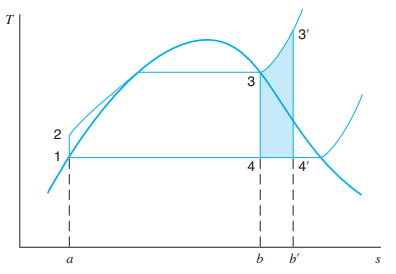
\includegraphics[width=0.4\textwidth]{./images/efeito-vapor.png}
	\caption{Efeito do superaquecimento do vapor sobre o rendimento do ciclo Rankine}
	\label{fig:efeito-vapor}
	\fonte{\cite{borgnakke-2020}}
\end{figure}

\subsubsection{Efeito da Pressão Máxima do Vapor}

A Figura \ref{fig:efeito-max-vapor} ilustra o impacto do aumento da pressão máxima do vapor. Mantendo-se constantes a temperatura máxima e a pressão de saída da turbina, o calor rejeitado diminui com a área b'-4'-4-b-b'. O trabalho líquido aumenta com a área hachurada simples e diminui com a área duplamente hachurada. O rendimento do ciclo aumenta com o aumento da pressão, pois o calor rejeitado diminui e a temperatura média de fornecimento de calor aumenta

\begin{figure}[h]
	\centering
	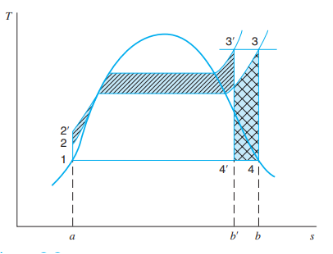
\includegraphics[width=0.4\textwidth]{./images/efeito-max-vapor.png}
	\caption{Efeito da pressão máxima do vapor sobre o rendimento do ciclo Rankine}
	\label{fig:efeito-max-vapor}
	\fonte{\cite{borgnakke-2020}}
\end{figure}

A Figura \ref{fig:efeito-pressao-temperatura} mostra como a pressão e a temperatura afetam o trabalho do ciclo Rankine. Já a Figura \ref{fig:efeito-pressao-temperatura-eficiencia} apresenta a influência dessas variáveis na eficiência do ciclo. Ambas destacam os efeitos combinados das variáveis.

\begin{figure}[h]
	\centering
	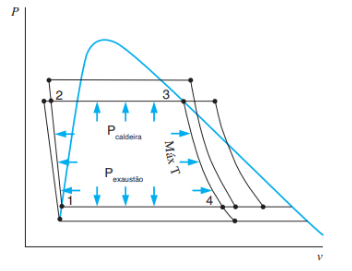
\includegraphics[width=0.4\textwidth]{./images/efeito-pressao-temperatura.png}
	\caption{Efeito da pressão e da temperatura no trabalho do ciclo Rankine}
	\label{fig:efeito-pressao-temperatura}
	\fonte{\cite{borgnakke-2020}}
\end{figure}

\begin{figure}
	\centering
	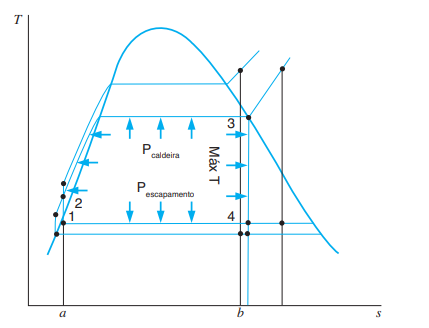
\includegraphics[width=0.4\textwidth]{./images/efeito-pressao-temperatura-eficiencia.png}
	\caption{Efeito da pressão e da temperatura na eficiência do ciclo Rankine}
	\label{fig:efeito-pressao-temperatura-eficiencia}
	\fonte{\cite{borgnakke-2020}}
\end{figure}

Esses três fatores combinados podem otimizar o ciclo Rankine, desde que o projeto evite problemas como erosão das palhetas da turbina devido a altos níveis de umidade.
Além dessas considerações, observamos que o ciclo é representado por quatro processos conhecidos (dois isobáricos e dois isentrópicos) que se desenrolam entre os quatro estados, abrangendo um total de oito características. Assumindo que o estado 1 seja um estado líquido saturado (x1 = 0), precisamos definir três parâmetros (8-4-1). A pressão operacional é controlada fisicamente pela alta pressão produzida pela bomba, P2 = P3, o superaquecimento para T3 (ou x3 = 1, se não houver superaquecimento) e a temperatura do condensador T1, que é o resultado da transferência de calor que acontece \cite{borgnakke-2020}.

\subsection{Interpretação Dos Efeito Das Pressões Da Caldeira E Do Condensador}

A Figura \ref{fig:efeitos-caldeira} exibe dois ciclos ideais submetidos à mesma pressão. Contudo, com pressões distintas na caldeira. Conforme a análise, a temperatura média do calor adicionado é maior no ciclo de pressão mais elevada 1' - 2' - 3' - 4' - 1' do que no ciclo 1 - 2 - 3 - 4 - 1. Portanto, o aumento da pressão na caldeira do ciclo ideal de Rankine tende a eficiência térmica.

\begin{figure}[h]
	\centering
	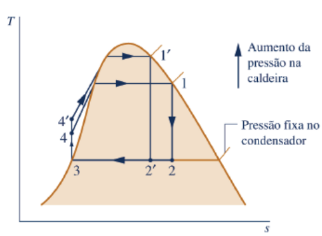
\includegraphics[width=0.4\textwidth]{./images/efeitos-caldeira.png}
	\caption{Efeitos da variação das pressões de operação do ciclo ideal Rankine na caldeira}
	\label{fig:efeitos-caldeira}
	\fonte{\cite{moran-2018}}
\end{figure}

A Figura \ref{fig:efeito-condensador} ilustra dois ciclos com pressões idênticas na caldeira, mas com duas pressões distintas no condensador. Um condensador funciona sob a pressão atmosférica, enquanto o outro opera sob uma pressão inferior à atmosfera. Para os ciclos 1-2-3-4-1 que condensam sob pressão atmosférica, a temperatura de rejeição de calor é de 100 °C (212 °F). A temperatura do calor devolvido para o ciclo de pressão mais baixa 1 - 2"- 3"- 4"- 1 é menor, resultando em uma maior eficiência térmica para este ciclo. Portanto, conclui-se que a redução da pressão no compressor tende a incrementar a eficiência térmica.

\begin{figure}[h]
	\centering
	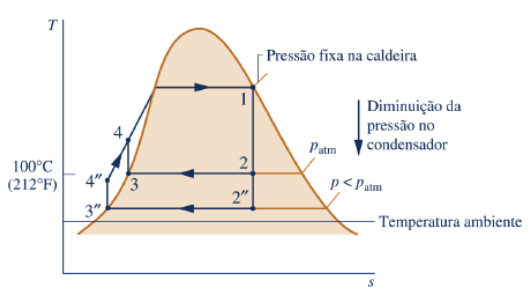
\includegraphics[width=0.5\textwidth]{./images/efeito-condensador.png}
	\caption{Efeitos da variação das pressões de operação do ciclo ideal Rankine no condensador}
	\label{fig:efeito-condensador}
	\fonte{\cite{moran-2018}}
\end{figure}

O condensador opera com a pressão de saturação equivalente à temperatura ambiente, pois esta é a temperatura ideal para a dissipação de calor para as proximidades. A finalidade de manter a pressão de exaustão mais baixa possível na turbina é a principal razão para a inclusão do condensador em uma instalação de potência. A caldeira poderia ser abastecida com água líquida à pressão atmosférica por meio da bomba, enquanto o vapor poderia ser liberado diretamente no ar ao sair da turbina. No entanto, ao incorporar um condensador, que opera a vapor a uma pressão inferior à atmosférica, a turbina terá uma área de pressão mais baixa onde será feita a descarga, o que resultará em um aumento do trabalho líquido da eficiência térmica. Incorporando um condensador adicional, o fluido de trabalho funcionará em circuito fechado, garantindo uma circulação constante do fluido de trabalho.

\subsection{Efeito da temperatura na eficiência térmica}

Basicamente o ciclo ideal Rankine consiste em processos onde existem reversibilidades internas, o que nos possibilita obter uma expressão para eficiência térmica em função das temperaturas médias durante o processo de interação térmica. A eficiência térmica do ciclo ideal Rankine é expressa pela equação \ref{eq:eficiencia-termica-temperatura}.

\begin{equation}
	\eta_{ideal} = 1 - \frac{T_{sai}}{T_{ent}}
	\label{eq:eficiencia-termica-temperatura}
\end{equation}

Pode-se concluir que a eficiência térmica do ciclo ideal tende a aumentar quando a temperatura média pela qual a energia é adicionada por transferência de calor aumenta ou a temperatura pela qual a energia rejeitada diminui.

\section{Ciclos de Rankine Modificados}

\subsection{Tipos de modificações}

O ciclo de Rankine pode ser modificado de várias maneiras para melhorar sua eficiência e desempenho. As modificações mais comuns incluem o superaquecimento, o reaquecimento e a regeneração térmica. Cada uma dessas técnicas tem o objetivo de aumentar a eficiência térmica do ciclo, reduzindo as perdas de calor e melhorando a qualidade do vapor na saída da turbina.

\subsubsection{Reaquecimento}

O ciclo Rankine com reaquecimento foi projetado para aproveitar o aumento de rendimento proporcionado por pressões mais altas, evitando umidade excessiva nos estágios de baixa pressão da turbina. Conforme ilustrado na Figura \ref{fig:reaquecimento}, o vapor inicialmente se expande até uma pressão intermediária na turbina, sendo reaquecido na caldeira antes de expandir novamente até a pressão de saída. Embora o diagrama T-s demonstre que o reaquecimento proporciona um pequeno ganho de rendimento devido à pequena variação na temperatura média de fornecimento de calor, sua principal vantagem reside na redução da umidade nos estágios finais da turbina. O autor destaca ainda que, caso os metais permitam um superaquecimento adequado do vapor até 3', o ciclo Rankine simples seria mais eficiente que o ciclo com reaquecimento, tornando este último desnecessário \cite{borgnakke-2020}.

\begin{figure}[h]
	\centering
	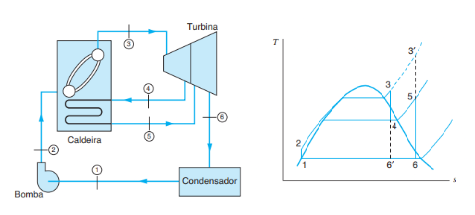
\includegraphics[width=0.65\textwidth]{./images/reaquecimento.png}
	\caption{Ciclo Rankine com reaquecimento}
	\label{fig:reaquecimento}
	\fonte{\cite{borgnakke-2020}}
\end{figure}

\subsubsection{Regeneração}

O ciclo Rankine regenerativo é uma importante variação que utiliza aquecedores da água de alimentação para melhorar a eficiência do sistema. Como mostrado na Figura \ref{fig:regerenacao}, no ciclo sem superaquecimento, o fluido de trabalho é aquecido na fase líquida entre os estados 2 e 2', com uma temperatura média significativamente menor em comparação ao processo de vaporização (2'-3). Isso resulta em uma temperatura média de transferência de calor inferior à do ciclo de Carnot (1'-2'-3-4-1), acarretando um rendimento menor. No ciclo regenerativo, o fluido entra na caldeira em um estado intermediário entre 2 e 2', aumentando a temperatura média de fornecimento de calor e, consequentemente, o rendimento do ciclo \cite{borgnakke-2020}.

\begin{figure}[h]
	\centering
	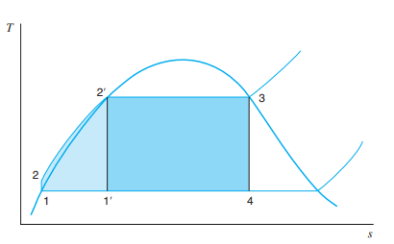
\includegraphics[width=0.5\textwidth]{./images/regeneracao.png}
	\caption{Diagrama T-s que mostra a relação entre os rendimentos dos ciclos de Carnot e Rankine.}
	\label{fig:regerenacao}
	\fonte{\cite{borgnakke-2020}}
\end{figure}

O ciclo regenerativo ideal, como ilustrado na Figura \ref{fig:regenerativo}, apresenta uma característica singular em comparação ao ciclo Rankine. Após a saída da bomba, o líquido circula ao redor da carcaça da turbina em sentido contrário ao do vapor, permitindo a transferência de calor do vapor para o líquido de forma teoricamente reversível. Nesse cenário ideal, a linha 4-5 no diagrama T-s, que representa o escoamento do vapor pela turbina, é paralela à linha 1-2-3, que indica o processo de bombeamento e o escoamento do líquido ao redor da turbina. As áreas 2-3-b-a-2 e 5-4-d-c-5 são congruentes e representam o calor transferido entre vapor e líquido. Esse ciclo apresenta rendimento térmico equivalente ao do ciclo de Carnot, já que a área 1-5-c-a-1 é igual à área de calor rejeitado do ciclo de Carnot \cite{borgnakke-2020}.

\begin{figure}[h]
	\centering
	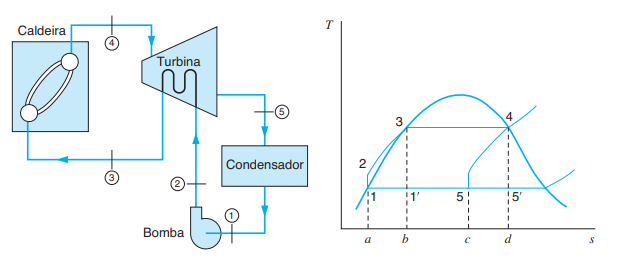
\includegraphics[width=0.65\textwidth]{./images/regenerativo.png}
	\caption{Ciclo Rankine regenerativo ideal}
	\label{fig:regenerativo}
	\fonte{\cite{borgnakke-2020}}
\end{figure}

Na prática, no entanto, a implementação desse ciclo ideal é inviável devido à dificuldade de realizar uma transferência de calor eficiente na turbina e ao aumento significativo da umidade do vapor na saída. O ciclo regenerativo real, mostrado na Figura \ref{fig:reg-aquecedor}, resolve essa limitação com a extração de parte do vapor parcialmente expandido na turbina, que é direcionado a aquecedores da água de alimentação. O líquido condensado é bombeado para se misturar ao vapor extraído, resultando em uma mistura saturada no estado 3. Para atingir a pressão da caldeira, uma segunda bomba é necessária. A vantagem principal desse ciclo é o aumento da temperatura média na qual o calor é fornecido ao fluido de trabalho, melhorando a eficiência térmica em comparação ao ciclo Rankine convencional \cite{borgnakke-2020}.

\begin{figure}[h]
	\centering
	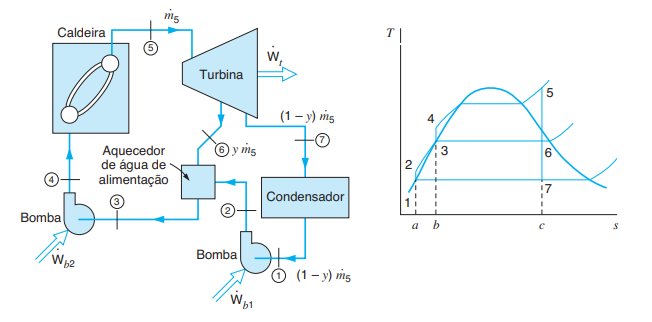
\includegraphics[width=0.65\textwidth]{./images/regenerativo-aquecedor.png}
	\caption{Ciclo regenerativo com aquecedor de água de alimentação de mistura}
	\label{fig:reg-aquecedor}
	\fonte{\cite{borgnakke-2020}}
\end{figure}

\subsubsection{Cogeração}




% ---
% Finaliza a parte no bookmark do PDF, para que se inicie o bookmark na raiz
% ---
\bookmarksetup{startatroot}%
% ---

% ---
% Conclusão
% ---
\section{Considerações finais}

% ----------------------------------------------------------
% ELEMENTOS PÓS-TEXTUAIS
% ----------------------------------------------------------
\postextual

% ----------------------------------------------------------
% Referências bibliográficas
% ----------------------------------------------------------
\clearpage
\bibliography{references}


\end{document}
